\documentclass[draft]{article}
%\documentclass{article}
\usepackage[utf8]{inputenc}
\usepackage[T1]{fontenc}
\usepackage{authblk}
\usepackage{hyperref}
\usepackage{bookmark}
\usepackage[margin=1in]{geometry}
%\usepackage{fullpage}
\usepackage[kerning,tracking,spacing,selected,final]{microtype}
\usepackage{minted}
\usepackage{listings}
\usepackage[position=top,skip=0pt]{caption}
\usepackage[position=top,skip=0pt]{subcaption}
\usepackage{varioref}
\usepackage[capitalise]{cleveref}
\usepackage{paralist}
%\usepackage{pslatex}
\usepackage{tikz}
\usepackage{ifdraft}
\usepackage[backend=biber,sortcites,datezeros=false]{biblatex}

\synctex=1
\addbibresource{proposal.bib}

\ifdraft{
	\usepackage{fix-cm}
	\usepackage{draftwatermark}
	\SetWatermarkLightness{0.85}
	\usepackage{xspace}
	\newcommand{\todoautocite}{(\textbf{TODO: Citation})\xspace}
}{}

\DeclareCaptionFormat{normal}{\normalsize#1#2#3\par}
\DeclareCaptionLabelFormat{bold}{\textbf{#1 #2}}
\DeclareCaptionLabelFormat{bold}{\textbf{#1 #2}}
\captionsetup{labelformat=bold,format=normal}
\DeclareCaptionLabelFormat{bold-sub}{\normalsize\textbf{(#2)}}
\captionsetup[sub]{labelformat=bold-sub,format=normal}

%\usepackage{setspace}
%\doublespacing
\microtypecontext{spacing=nonfrench}
\lstset{language=C}
%\pagestyle{empty}

%\title{Introspection via Self Debugging}
%\author{Russell Harmon \\ \url{reh5586@cs.rit.edu}}
%\affil{Rochester Institute of Technology \\ Computer Science}
%\date{}

\begin{document}

%\maketitle
\twocolumn[
	\centerline{\Large \bf Introspection via Self Debugging}
	\medskip
	\centerline{Russell Harmon}
	\centerline{\url{reh5586@cs.rit.edu}}
	\centerline{Rochester Institute of Technology}
	\centerline{Computer Science}
	\bigskip
]

\section{Introduction}
The omnipresent support for introspection in modern programming languages
indicates the usefulness of the tool. \autocite{java-reflect, ruby-introspect,
python-introspect, perl-introspect} Unfortunately, C, which is one of the most
pervasive programming languages and the foundation of nearly every modern
operating system, does not support introspection.

I propose to bring introspection to the C language via a novel application of an
old tool: the debugger. Debuggers have long had access to the type and naming
information which is needed for introspection. On most UNIX platforms, this is
accomplished by the debugger reading any DWARF \autocite{dwarf} symbols which may
be present in the target binary. These symbols can be leveraged to gain the
information which is needed to create a full-featured introspection API.

\section{Rationale}
One of the motivating factors for any language introducing introspection as a
feature is the following use case:

\begin{quotation}
	You are tasked with changing the save game format of a popular 1980s style
	terminal based game from a binary format composed of writing the structs
	which compose the game state to disk to a more flexible JSON format. After
	investigation, you discover that in order to do this, you can use the
	Jansson \autocite{jansson} C library to produce JSON. In order to do so, you
	invoke variants of the \texttt{json\_object\_set} function as given by the
	following prototype:
	\begin{minted}[gobble=2,tabsize=2]{c}
		int json_object_set(
			json_t *object,
			const char *key,
			json_t *value
		);
	\end{minted}
	You notice that \texttt{json\_object\_set} takes as parameters the name and
	value of the field to be written necessitating you writing a separate
	\texttt{json\_object\_set} call for every field of every struct which is to
	be written. After considering the literally thousands of fields across the
	nearly three hundred structs in the game you give up in frustration.
\end{quotation}

Clearly, it is a significant convenience to developers to be able to write code
which is able to introspect upon data in a meta-programming style.

\section{Introspection in Current Programming Languages}
Introspection is found in many of the programming languages commonly used today
including Java \autocite{java-reflect}, Ruby \autocite{ruby-introspect},
Python \autocite{python-introspect}, Perl \autocite{perl-introspect} and a
limited form of introspection in C++ \autocite{cpp-rtti}. The various approaches
to introspection differ in implementation detail; some receiving introspection
as a direct consequence of the way they implement objects while some provide it
as part of the standard library. Despite this, they all provide approximately
the same set of features. It is by these features that introspection can be
defined, rather than the details of how the features are implemented.

Two features are generally required in order to be considered introspection;
\emph{type} and \emph{function enumeration}. In Java, the availability of
\emph{type enumeration} means that a program can retrieve the name of an object
and enumerate the fields of that object, retrieving strings representing their
names, types and it's values, including the object's methods. \emph{Function
enumeration} can then be performed on the methods of an object giving access to
information about the return type and argument types, including the names of the
arguments.

Existing attempts to add introspection to C++ frequently require a separate
description of the object to be implemented which is generated using either a
separate parser \autocite{seal-cpp} or using a complementary \emph{metadata object}
\autocite{deBayser:2012:SRT:2415308.2415317} and have the limitation that objects
which come from external libraries cannot be introspected. Our implementation of
introspection will neither have this library boundary limitation nor require
external tools or additional objects in order to operate.

\section{Debugging in C}
There already exist a number of tools for interactive debugging of C programs.
Some of the more well known ones include GDB \autocite{gdb}, WinDBG, Visual Studio's
debugger and LLDB. \autocite{lldb} Traditionally, these debuggers have been used
interactively via the command line, although more recently debuggers such as the
one embedded within Visual Studio integrate into an IDE.

An understanding of debugging in general, and about LLDB specifically are
crucial to the understanding of this proposal, so some time will be spent
explaining debugging.

The first step in debugging a program is the creation of a debuggable binary.
This is accomplished by instructing the compiler to insert debugging symbols,
commonly DWARF on UNIX platforms, into the binary. Interactive debugging is
possible without these symbols, but becomes difficult. (TODO: Perhaps add more
here as to why debugging without symbols is hard?)

The DWARF symbols provide LLDB with information about the variables and
functions in the program and enables LLDB to determine the line number which
produced a particular sequence of instructions.

\subsection{LLDB}
\Vref{fig:debugging} shows a simple debugging session using LLDB. In it, a test
program is launched and the value of a stack-local variable is printed. Take
note that LLDB is aware that the type of \texttt{foo.bar} is \texttt{char *}. In
fact, most debuggers make available to their users nearly all of the type
information which is available to the programmer writing the original source file.

\begin{figure*}[p]
	\begin{verbatim}
		Current executable set to './a.out' (x86_64).
		(lldb) breakpoint set -n main
		Breakpoint created: 1: name = 'main', locations = 1
		(lldb) run
		Process 10103 launched: './a.out' (x86_64)
		Process 10103 stopped
		* thread #1: tid = 0x1c03, 0x0000000100000f60 a.out`main + 16 at a.c:6
		    frame #0: 0x0000000100000f60 a.out`main + 16 at a.c:6
		   3    };
		   4    int main() {
		   5            struct foo foo;
		-> 6            foo.bar = "Hello World!";
		   7    }
		(lldb) next
		Process 10103 stopped
		* thread #1: tid = 0x1c03, 0x0000000100000f64 a.out`main + 20 at a.c:7
		    frame #0: 0x0000000100000f64 a.out`main + 20 at a.c:7
		   4    int main() {
		   5            struct foo foo;
		   6            foo.bar = "Hello World!";
		-> 7    }
		(lldb) print foo.bar
		(char *) $0 = 0x0000000100000f66 "Hello World!"
		(lldb) exit
	\end{verbatim}
	\caption{Interactive Debugging with LLDB}
	\label{fig:debugging}
\end{figure*}

While type information is useful while interactively debugging a program, the
fact that LLDB is able to determine this information while the program is
running suggests that if a program can itself control LLDB, it could potentially
retrieve this type information about itself.

\begin{figure*}[p]
	\begin{verbatim}
		Process 12066 stopped
		* thread #1: tid = 0x1c03, 0x0000000100000f64 a.out`main + 20 at a.c:3
		    frame #0: 0x0000000100000f64 a.out`main + 20 at a.c:3
		   1    int main() {
		   2            void *baz = "Hello World!";
		-> 3    }
		(lldb) print baz
		(void *) $0 = 0x0000000100000f66
		(lldb) exit
	\end{verbatim}
	\caption{Static Type Information in Debuggers}
	\label{fig:static_introspection}
\end{figure*}

An important aspect of the type information which is available to LLDB is that
this information is purely static. The debugger knows only the type of the
variable being displayed, rather than the type of the data itself. This is in
stark contrast with other introspective languages where the type information is
carried with the data and can be recovered without any additional context. An
example of the result of this is shown in \vref{fig:static_introspection}.

\section{Related Work}
\emph{A System for Runtime Type Introspection in C++}
\autocite{deBayser:2012:SRT:2415308.2415317} discusses an approach to introspection
for C++ whereby metadata objects are created using macros which are expected to
be called at the definition of the object which is to be introspected.

\emph{The Seal C++ Reflection System} \autocite{seal-cpp} discusses an introspection
system for C++ which uses a metadata generation tool to create descriptor files
which contain the information needed for introspection.

\emph{Reflection for C++} \autocite{reflection-for-cpp} uses an approach very
similar to the one proposed here, but instead of using a debugger to retrieve
debugging information, it instead reads the debugging symbols directly. This
limits the API to only leveraging information that it can retrieve from the
debugging symbols themselves, as opposed to could be retrieved via interactive
debugging. This possibility is discussed in Section \ref{sec:future_work}.

C++, along with all the other languages supported by Microsoft's CLR can be
reflected upon by leveraging features exposed by the CLR. \autocite{clr-cpp}

\section{Approach \& Design}
By leveraging LLDB, I hope to create an API which allows a program to read the
DWARF symbols of any object file, shared library or executable; including
itself. The API which programmers will interact with should be complete enough
that the presence of LLVM should be completely hidden from the programmer. This
API should minimally allow introspection of scalar and pointer values,
typedef'ed values, structs, functions and struct members; allowing access to the
variable, struct member or function name, type name, size, struct member offset,
function arguments and return type.

LLDB's API is not designed to require attaching to a running process in order to
retrieve static debugging information which can be determined simply by
examining the symbols in the binary. If information which is not available
statically is needed, a running instance of the program can be started or
attached to. For the initial implementation of the introspective API, attaching
to the running program should not be necessary as all the introspective
information needed should be retrievable directly from the executable file's
debugging symbols. See Section \ref{sec:future_work} for future improvements
that debugging the running program could provide.

The code shown in \cref{fig:struct_introspect:code} is a simple example of a
feature which will be enabled by this API. In \cref{fig:struct_introspect:code},
a struct named \texttt{foo} is introspected upon in order to produce the output
shown in \cref{fig:struct_introspect:output}. Notice that although the API will
not directly provide a method to access the introspected data's value, it is
accessible indirectly via the \emph{offset} and \emph{size} fields which are
available.

\Cref{fig:introspective_api} shows a tentative partial API complete enough for
the example mentioned above and shown in \vref{fig:struct_introspect}. A program
would call \texttt{get\_type} in order to retrieve a \texttt{type\_t} whose
storage is managed by \texttt{get\_type}. This \texttt{type\_t} can then be used
to determine information such as the name or size of the type which it
represents by casting the \texttt{type\_t} to the appropriate concrete type as
indicated by the \texttt{type\_t.type} field.

\begin{figure}
	{
		\footnotesize
		\inputminted[tabsize=2]{c}{introspection.h}
	}
	\caption{Tentative Introspective API}
	\label{fig:introspective_api}
\end{figure}

\begin{figure}
	\begin{subfigure}{\linewidth}
		{
			\footnotesize
			\inputminted[tabsize=2]{c}{struct_introspect.c}
		}
		\caption{Introspective code}
		\label{fig:struct_introspect:code}
	\end{subfigure}
	\begin{subfigure}{\linewidth}
		{
			\footnotesize
			\begin{verbatim}
				(foo) {
				  .str = (string_t) "Hello World!"
				  .i = (int) 6666
				}
			\end{verbatim}
		}
		\caption{Output from introspective code}
		\label{fig:struct_introspect:output}
	\end{subfigure}
	\caption{Introspection Using this API}
	\label{fig:struct_introspect}
\end{figure}

\subsection{The LLDB API}
Currently, LLDB is a relatively new project, and is only sparsely documented. It
does however have example code of the use of it's API. From reading the sources
to LLDB, there exists an \texttt{SBType} class which represents a type. These
types include struct, function and primitive types. Using a \texttt{SBType}, all
the information needed for a fully featured introspective API can be retrieved.

\section{Limitations}
This style of introspection is slightly more limited than the classic style of
introspection whereby an object carries it's own type information. Instead, the
type of a \emph{value} must be specified either by the type of it's
\emph{variable}, or explicitly by passing a string representation of it's type
to the introspective API. The only limitation this \emph{static introspection}
should impose on the programmer is that an unknown \lstinline|void *| type
cannot be introspected.

Under current plans, the programmer will have to provide the desired type as a
string to the \texttt{get\_type} function. It is however desirable to be able to
use any expression as the argument to \texttt{get\_type}. In order to accomplish
this, a running debugger will need to be attached to the program in
order to determine the result type of the expression. Future work may provide
this feature.

Although not strictly a limitation, many programmers will likely want to
introspect strings as such, rather than as the \lstinline|char *| type.
Unfortunately, since there is no typing difference between a C string and a
pointer to one or more chars, this introspective API will be unable to determine
the difference between the two.  The example code shown in
\vref{fig:struct_introspect:code} works around this issue by creating a typedef
of \lstinline|char *| to \lstinline|string_t|.

\section{Timeline \& Completion}
Beyond design and implementation of the introspective API, completion of this
project would be measured by the following criteria:
\begin{inparaenum}[\itshape a\upshape)]
\item
	code which is similar in structure to \vref{fig:struct_introspect:code}
	is able to produce the output shown in \vref{fig:struct_introspect:output}
\item
	a proof of concept \texttt{abort\_with\_stacktrace()} function which when
	invoked prints a complete stack trace to standard error and exits and
\item
	the release of the source code in a usable, fully documented form on the
	internet.
\end{inparaenum}

The work to create an introspective API is expected to take approximately three
to four months. This is expected to occur between the months of April and
August.

\begin{figure}
	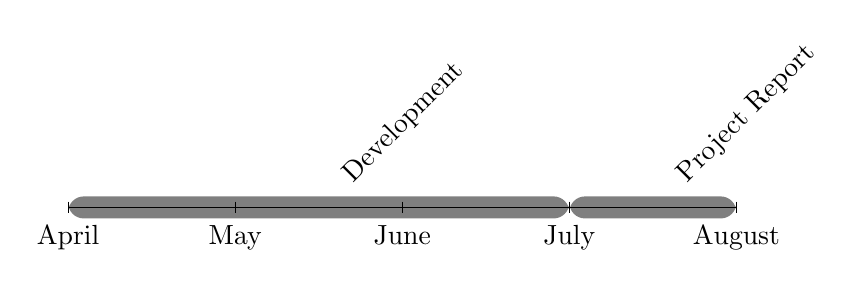
\begin{tikzpicture}[scale=.7]
		\noindent
		\newcommand{\tlwidth}{\columnwidth}
		%draw horizontal line
		\draw (0,0) -- (\tlwidth,0);

		%draw vertical lines
		\foreach \x in {0,.25,.5,.75,1}
			\draw (\x\tlwidth,3pt) -- (\x\tlwidth,-3pt);

		%draw nodes
		\draw (0,0) node[above=3pt] {}; % Force space above
		\draw (0,0) node[below=3pt] {April};
		\draw (.25\tlwidth,0) node[below=3pt] {May};
		\draw (.5\tlwidth,0) node[below=3pt] {June};
		\draw (.75\tlwidth,0) node[below=3pt] {July};
		\draw (1\tlwidth,0) node[below=3pt] {August};

		\newcommand{\event}[3][e] {
			\ifx #1e
				\draw[fill=black,draw=none,opacity=0.5]
					(#2\tlwidth,0) circle (.2cm)
					node[opacity=1,rotate=45,right=.4cm] {#3};
			\else
				\draw[fill=black,draw=none,opacity=0.5,rounded corners=.2cm]
					(#1\tlwidth,-.2cm) rectangle
					node[opacity=1,rotate=45,right=.4cm] {#3} (#2\tlwidth,.2cm);
			\fi
		}
		\event[0]{.75}{Development}
		\event[.75]{1}{Project Report}

		\ifdraft{
			\draw[red] (current bounding box.south west) rectangle (current bounding box.north east);
		}{}
	\end{tikzpicture}
	\caption{Completion Timeline}
	\label{fig:completion_timeline}
\end{figure}

As shown in \vref{fig:completion_timeline}, I expect the actual programming
portion of the project to take until July and the writing of the thesis to take
until August. I expect to be able to defend by the beginning of the first
academic semester of 2013.

\section{Future Work}
\label{sec:future_work}
In order to enable the passing of an expression to \texttt{get\_type}, it should
be possible to spawn a \emph{debugger control thread}, which receives requests
from other threads. These requests would be serviced by attaching to the
requesting thread, manipulating the debugger to retrieve the type of the passed
in variable, and finally passing that information back to the requesting thread.
This design is chosen due to the anticipated limitation in LLVM that you will be
unable to attach to your own thread.

It should be possible to extend this API to operate with other debuggers (e.x.
\texttt{gdb}) possibly even on other platforms (e.x. \texttt{windbg} on
Windows). Currently, efforts will be focused on features of the introspective
API before portability is considered.

\onecolumn
\printbibliography

\end{document}

% vim:tw=80 spell
